%%%%%%%%%%%%%%%%%%%%%%%%%%%%%%%%%%%%%%%%%
% Compact Laboratory Book
% LaTeX Template
% Version 1.0 (4/6/12)
%
% This template has been downloaded from:
% http://www.LaTeXTemplates.com
%
% Original author:
% Joan Queralt Gil (http://phobos.xtec.cat/jqueralt) using the labbook class by
% Frank Kuster (http://www.ctan.org/tex-archive/macros/latex/contrib/labbook/)
%
% License:
% CC BY-NC-SA 3.0 (http://creativecommons.org/licenses/by-nc-sa/3.0/)
%
% Important note:
% This template requires the labbook.cls file to be in the same directory as the
% .tex file. The labbook.cls file provides the necessary structure to create the
% lab book.
%
% The \lipsum[#] commands throughout this template generate dummy text
% to fill the template out. These commands should all be removed when 
% writing lab book content.
%
% HOW TO USE THIS TEMPLATE 
% Each day in the lab consists of three main things:
%
% 1. LABDAY: The first thing to put is the \labday{} command with a date in 
% curly brackets, this will make a new section showing that you are working
% on a new day.
%
% 2. EXPERIMENT/SUBEXPERIMENT: Next you need to specify what 
% experiment(s) and subexperiment(s) you are working on with a 
% \experiment{} and \subexperiment{} commands with the experiment 
% shorthand in the curly brackets. The experiment shorthand is defined in the 
% 'DEFINITION OF EXPERIMENTS' section below, this means you can 
% say \experiment{pcr} and the actual text written to the PDF will be what 
% you set the 'pcr' experiment to be. If the experiment is a one off, you can 
% just write it in the bracket without creating a shorthand. Note: if you don't 
% want to have an experiment, just leave this out and it won't be printed.
%
% 3. CONTENT: Following the experiment is the content, i.e. what progress 
% you made on the experiment that day.
%
%%%%%%%%%%%%%%%%%%%%%%%%%%%%%%%%%%%%%%%%%

%----------------------------------------------------------------------------------------
%	PACKAGES AND OTHER DOCUMENT CONFIGURATIONS
%----------------------------------------------------------------------------------------                               

\documentclass[fontsize=11pt, % Document font size
                             paper=a4, % Document paper type
                             oneside, % Shifts odd pages to the left for easier reading when printed, can be changed to oneside
                             captions=tableheading,
                             index=totoc,
                             hyperref]{labbook}
 
\usepackage[bottom=10em]{geometry} % Reduces the whitespace at the bottom of the page so more text can fit

\usepackage[english]{babel} % English language
\usepackage{lipsum} % Used for inserting dummy 'Lorem ipsum' text into the template

%\usepackage[utf8]{inputenc} % Uses the utf8 input encoding
\usepackage[T1]{fontenc} % Use 8-bit encoding that has 256 glyphs

\usepackage[osf]{mathpazo} % Palatino as the main font
\linespread{1.05}\selectfont % Palatino needs some extra spacing, here 5% extra
\usepackage[scaled=.88]{beramono} % Bera-Monospace
\usepackage[scaled=.86]{berasans} % Bera Sans-Serif

\usepackage{booktabs,array} % Packages for tables

\usepackage{amsmath} % For typesetting math
\usepackage{graphicx} % Required for including images
\usepackage{etoolbox}
\usepackage[norule]{footmisc} % Removes the horizontal rule from footnotes
\usepackage{lastpage} % Counts the number of pages of the document

\usepackage[dvipsnames]{xcolor}  % Allows the definition of hex colors
\definecolor{titleblue}{rgb}{0.16,0.24,0.64} % Custom color for the title on the title page
\definecolor{linkcolor}{rgb}{0,0,0.42} % Custom color for links - dark blue at the moment

\addtokomafont{title}{\Huge\color{titleblue}} % Titles in custom blue color
\addtokomafont{chapter}{\color{OliveGreen}} % Lab dates in olive green
\addtokomafont{section}{\color{Sepia}} % Sections in sepia
\addtokomafont{pagehead}{\normalfont\sffamily\color{gray}} % Header text in gray and sans serif
\addtokomafont{caption}{\footnotesize\itshape} % Small italic font size for captions
\addtokomafont{captionlabel}{\upshape\bfseries} % Bold for caption labels
\addtokomafont{descriptionlabel}{\rmfamily}
\setcapwidth[c]{10cm} % Right align caption text c is "center", l is "left", r is "right"
\setkomafont{footnote}{\sffamily} % Footnotes in sans serif

\deffootnote[4cm]{4cm}{1em}{\textsuperscript{\thefootnotemark}} % Indent footnotes to line up with text

\DeclareFixedFont{\textcap}{T1}{phv}{bx}{n}{1.5cm} % Font for main title: Helvetica 1.5 cm
\DeclareFixedFont{\textaut}{OT1}{phv}{bx}{n}{0.8cm} % Font for author name: Helvetica 0.8 cm

\usepackage[nouppercase,headsepline]{scrpage2} % Provides headers and footers configuration
\pagestyle{scrheadings} % Print the headers and footers on all pages
\clearscrheadfoot % Clean old definitions if they exist

\automark[chapter]{chapter}
\ohead{\headmark} % Prints outer header

\setlength{\headheight}{25pt} % Makes the header take up a bit of extra space for aesthetics
\setheadsepline{.4pt} % Creates a thin rule under the header
\addtokomafont{headsepline}{\color{lightgray}} % Colors the rule under the header light gray

\ofoot[\normalfont\normalcolor{\thepage\ |\  \pageref{LastPage}}]{\normalfont\normalcolor{\thepage\ |\  \pageref{LastPage}}} % Creates an outer footer of: "current page | total pages"

% These lines make it so each new lab day directly follows the previous one i.e. does not start on a new page - comment them out to separate lab days on new pages
\makeatletter
\patchcmd{\addchap}{\if@openright\cleardoublepage\else\clearpage\fi}{\par}{}{}
\makeatother
\renewcommand*{\chapterpagestyle}{scrheadings}

% These lines make it so every figure and equation in the document is numbered consecutively rather than restarting at 1 for each lab day - comment them out to remove this behavior
\usepackage{chngcntr}
\counterwithout{figure}{labday}
\counterwithout{equation}{labday}

% Hyperlink configuration
\usepackage[
    pdfauthor={}, % Your name for the author field in the PDF
    pdftitle={Laboratory Journal}, % PDF title
    pdfsubject={}, % PDF subject
    bookmarksopen=true,
    linktocpage=true,
    urlcolor=linkcolor, % Color of URLs
    citecolor=linkcolor, % Color of citations
    linkcolor=linkcolor, % Color of links to other pages/figures
    backref=page,
    pdfpagelabels=true,
    plainpages=false,
    colorlinks=true, % Turn off all coloring by changing this to false
    bookmarks=true,
    pdfview=FitB]{hyperref}

\usepackage[stretch=10]{microtype} % Slightly tweak font spacing for aesthetics

%\setlength\parindent{0pt} % Uncomment to remove all indentation from paragraphs

\usepackage{zhfontcfg}% Chinese fonts
\usepackage{indentfirst} % indention for Chinese
\setlength{\parindent}{2em}

\usepackage{algorithm}
\usepackage{algorithmicx}
\usepackage{algpseudocode}

%----------------------------------------------------------------------------------------
%	DEFINITION OF EXPERIMENTS
%----------------------------------------------------------------------------------------

% Template: \newexperiment{<abbrev>}[<short form>]{<long form>}
% <abbrev> is the reference to use later in the .tex file in \experiment{}, the <short form> is only used in the table of contents and running title - it is optional, <long form> is what is printed in the lab book itself

\newexperiment{学习情况}[学习情况]{学习情况}

\newexperiment{quicksort}[快速排序]{快速排序算法}
\newsubexperiment{para_qs_MPI}[快速排序MPI实现]{快速排序MPI实现}
\newsubexperiment{para_qs_OpenMP}[快速排序OpenMP实现]{快速排序OpenMP实现}
\newsubexperiment{para_qs_result}[实验结果与分析]{实验结果与分析}

%----------------------------------------------------------------------------------------

\begin{document}

%----------------------------------------------------------------------------------------
%	TITLE PAGE
%----------------------------------------------------------------------------------------

\title{\erhao\hei{学习情况} \\[1cm]  
\textaut{2014-4-11}}

\author{
    %\textaut{周永强 Yongqiang Zhou}\\ \\ % Your name
	\erhao{\hei{周永强}} \\[1cm]
	\fzqt{六院八队} % Your degree
}
\date{} % No date by default, add \today if you wish to include the publication date

\maketitle % Title page

\printindex
\tableofcontents % Table of contents

\newpage % Start lab look on a new page

\begin{addmargin}[0cm]{0cm} % Makes the text width much shorter for a compact look

\pagestyle{scrheadings} % Begin using headers

%----------------------------------------------------------------------------------------
%	LAB BOOK CONTENTS
%----------------------------------------------------------------------------------------
\labday{说明}
\experiment{学习情况}
\indent 这两周主要还是在上课,清明跑出去玩了两天,这篇报告是根据自己的课程《高级并行程序设计》来写的。上次师门报告的时候听师兄讲了一些工具的使用,有些是我知道的,有些是我不知道的但是却感兴趣的,于是这两周有相当一部分时间花在了工具的学习和使用上。\\
\indent 期间学习了\en{\LaTeX{}}排版,以前只是知道有这个工具,但是没有用过,这次集中学习了一下,这篇报告就是用其排版而成,当然我不是从头做的,而是基于网上提供的一个模板。\en{\LaTeX{}}功能很多,我着重学习了比较常用的,也是自己当前需要使用的功能,包括:数学公式、伪代码书写、图片插入等。其次学习\en{gnuplot}绘图工具用于绘制常用数据分析图。本篇报告中的折线图就是用\en{gnuplot}绘制的。\\
\indent 结合课程需要,这两周在学习\en{MPI}编程,了解并行编程模型。目前对于并行编程我还处于入门阶段,后续我准备继续学习\en{MPI},以及\en{OpenMP},为以后的学习和工作打下基础,毕竟我当前并行方面的知识比较缺乏。下文中给出的是一个快速排序算法的实例,为了说明这两周的学习情况,由于时间不够用(主要是我懒),所以\en{OpenMP}版本程序没有写。\\
\indent 实验室那边这两周去的比较少,期间假期外出的缘故为一,其次则是课程这边也需要花不少时间。目前那边的情况是基本功能实现了,但是性能还跟不上去,达不到要求,主要是为并行程序设计把握的不好,这段时间我再想想办法改进。
%----------------------------------------------------------------------------------------
% 实验一:快速排序算法
%----------------------------------------------------------------------------------------
\labday{快速排序}
\indent 本节中先给出快速排序的串行化算法,然后对算法进行分析,引出并行的快速排序算法,并且分别使用\en{MPI}和\en{OpenMP}实现并行的快速排序,最后对算法的性能进行评估,给出评价和结果分析。
%评估主要根据加速比等性能指标,绘制图表

%-----------------------------------------

\experiment{quicksort}
%算法的串行伪代码,并行化分析并行代码
\indent 快速排序是一种基本的排序算法,其时间复杂度为$O(n\log{n})$,它的基本思想是:对于给定的无序序列$R[1,n]$,从中选取一个元素作为“标兵”(一般选取第一个元素或最后一个元素),以“标兵”为基准将序列划分为两个子序列$R[1,i-1]$和$R[i,n]$,且左边的无序子区中记录的所有关键字均小于等于基准的关键字,右边的无序子区中记录的所有关键字均大于等于基准的关键字,当子序列不空时,递归调用子上述过程,程序运行结束时,序列有序。\\
\begin{algorithm}
\caption{快速排序算法}\label{ser_quicksort}
\begin{algorithmic}[1]
\Function{\color{titleblue}{quicksort}}{$data, i, j$}\Comment{quicksort from i to j}
   \If{$i<j$}
       \State $r \gets$ partition($data, i, j$) 
   \EndIf
   \State quicksort($data, i, r-1$)
   \State quicksort($data, r+1, j$)
\EndFunction
\end{algorithmic}
\end{algorithm}
\indent 快速排序依赖划分操作,划分算法给出如下。
\begin{algorithm}
\caption{partition算法}\label{partition}
\begin{algorithmic}[1]
\Function{partition}{$data, k, l$}
   \State $pivo \gets data[l]$
   \State $i \gets k-l$ 
   \For {$j \gets k,l-1$}
       \If{$data[i] \le pivo$} %\le <= \ge is >=
           \State $i \gets i+1$
           \State exchange $data[i]$ and $data[j]$
       \EndIf
   \EndFor
   \State exchange $data[i+1]$ and $data[l]$
   \State return $i+1$
\EndFunction
\end{algorithmic}
\end{algorithm}\\
\indent 快速排序算法并行化的一个简单思想是,对每次划分过后所得到的两个序列分别使用两个处理器完成递归排序。例如对一个长为$n$的序列,首先划分得到两个长为$n/2$的序列,将其交给两个处理器分别处理;而后进一步划分得到四个长为$n/4$的序列,再分别交给四个处理器处理;如此递归下去最终得到排序好的序列。
\begin{algorithm}
\caption{快速排序并行算法}\label{para_quicksort}
\begin{algorithmic}[1]
\Function{para\_quicksort}{$data, i, j, m, id$}
    \If{$(j-i) \le k || m = 0$}
        \State {$P_{id}:$ call quicksort($data, i, j$)}
    \Else
        \State {$P_{id} r = $ partition($data, i, j$)}
        \State $P_{id}:$ send $data[r+1, m-1]$ to $P_{id+2^{m-1}}$
        \State \Call{para\_quicksort}{$data, i, r-1, m-1, id$}
        \State \Call{para\_quicksort}{$data, r+1, j, m-1, id+2^{m-1}$}
        \State $P_{id}:$ send $data[r+1, m-1]$ back to $P_{id}$
    \EndIf
\EndFunction
\end{algorithmic}
\end{algorithm}

%-----------------------------------------

\subexperiment{para_qs_MPI}
%分析如何用mpi进行实现
\en{MPI}是\en{Message Passing Interface}的缩写,中译为消息传递接口,用于分布式内存系统的编程,在目前并行计算领域广为应用。\en{MPI}并不是一门编程语言,而是与编程语言库的形式提供,开发人员可以根据自己问题的需要,应用\en{MPI}进行并行编程。\\
\en{MPI}数据传送分为阻塞与非阻塞两种,通信方式有广播方式和点对点方式,快速排序中,由0号进程负责对数据进行初始化,然后将长度广播到其他的所用进程。限于篇幅,这里不再贴出源代码。
%-----------------------------------------

\subexperiment{para_qs_OpenMP}
%分析如何用openmp进行实现
%OpenMP实现的代码与说明
暂未实现
%-----------------------------------------

\subexperiment{para_qs_result}
%结论
\indent 程序的测试在我的个人笔记本上完成,\en{CPU}芯片为\en{Intel T6600}双核处理器,图中给出的是单个进程在执行并行快速排序时所耗用的时间。测试中选用定长的1000000条数据进行排序,分别统计了1,2,4,8个进程时在单个进程上排序所耗用的时间,这里没有算上通信所带来的开销。图中可以明确看出随着进程数的增加,单个进程上的并行快速排序时间在减少,而且当进程数增加到原来的两倍时,排序时间大约减为原来的一半。由此,除去通信的开销,并行程序的效率明显高于串行程序,当然这是以更高的硬件资源为代价的。
\begin{figure}[h!]
\centering
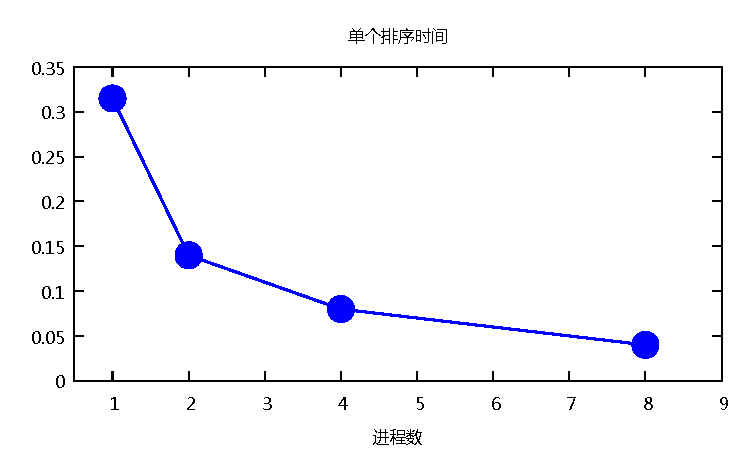
\includegraphics[scale=1,keepaspectratio=true]{analysis.pdf}
\caption{MPI结果分析图}
\label{fig:mpi_analysis}
\end{figure}

%----------------------------------------------------------------------------------------
% 实验二 Cannon方法的矩阵乘
%----------------------------------------------------------------------------------------
%\labday{矩阵相乘的Cannon方法}
%矩阵相互乘
%\experiment{Cannon方法的矩阵乘}

\end{addmargin}

%----------------------------------------------------------------------------------------
%	BIBLIOGRAPHY
%----------------------------------------------------------------------------------------

\begin{thebibliography}{9}

\bibitem{lamport94}
Leslie Lamport,
\emph{\LaTeX: A Document Preparation System}.
Addison Wesley, Massachusetts,
2nd Edition,
1994.

\bibitem{hello}
陈国良,
\emph{并行计算——结构算法编程}.
高等教育出版社,
1999.

\end{thebibliography}

%----------------------------------------------------------------------------------------

\end{document}
